\documentclass[pdftex,twocolumn,epjc3]{svjour3}          % twocolumn

\RequirePackage[T1]{fontenc}

\smartqed  % flush right qed marks, e.g. at end of proof

\RequirePackage{siunitx}
\RequirePackage{graphicx}
\RequirePackage{mathptmx}      % use Times fonts if available on your TeX system
\RequirePackage{flushend}
\RequirePackage[numbers,sort&compress]{natbib}
\RequirePackage[colorlinks,citecolor=blue,urlcolor=blue,linkcolor=blue]{hyperref}

\journalname{Eur. Phys. J. C}

\begin{document}

\title{Development of a MALTA2-Based Fast MAPS Tracker: Detector Design, Readout Firmware, and Performance Validation}

%\subtitle{Do you have a subtitle?\\ If so, write it here}

\author{Xuan Li \thanksref{e1,addr1}
        \and
        Joellen Renck \thanksref{addr1}
        \and
        Dien Nguyen \thanksref{e2,addr2}
        \and
        Lindsey Hessler \thanksref{addr2}
        \and
        Abhishek Abhishek \thanksref{addr2}
        \and
        Amelia Sandoval \thanksref{addr2,addr1} 
        \and
        Carlos Solans Sanchez \thanksref{e3,addr3}
        \and
        F. Kerem Isık \thanksref{addr4}
        \and
        Vlad Berlea \thanksref{e4, addr5}
        \and
        Lucian Fasselt \thanksref{e5, addr5}
        \and
        Cigdem Issever \thanksref{addr5}
        \and
        Steven Worm \thanksref{addr5}
}

%%=============================================================%%
%% GivenName	-> \fnm{Joergen W.}
%% Particle	-> \spfx{van der} -> surname prefix
%% FamilyName	-> \sur{Ploeg}
%% Suffix	-> \sfx{IV}
%% \author*[1,2]{\fnm{Joergen W.} \spfx{van der} \sur{Ploeg} 
%%  \sfx{IV}}\email{iauthor@gmail.com}
%%=============================================================%%

%\thankstext[$\star$]{t1}{Thanks to the title}
\thankstext{e1}{e-mail: xuanli@lanl.gov}
\thankstext{e2}{e-mail: dnguye41@utk.edu}
\thankstext{e3}{e-mail: carlos.solans@cern.ch}
\thankstext{e4}{e-mail: vlad.berlea@desy.de}
\thankstext{e5}{e-mail: lucian.fasselt@desy.de}
%\thankstext{e5}{e-mail: fuat.kerem@cern.ch}

\institute{Los Alamos National Laboratory, P. O. Box 1663, Los Alamos, United States\label{addr1}
          \and
          University of Tennessee, Knoxville, TN, USA\label{addr2}
          \and
          CERN, Geneva, Switzerland\label{addr3}
          \and
          Ankara University, Ankara, Turkey\label{addr4}
          \and
          Deutsches Elektronen-Synchrotron DESY, Zeuthen, Germany\label{addr5}
          %\emph{Present Address:} Street, City, Country\label{addr3}
}

\date{Received: date / Accepted: date}
% The correct dates will be entered by the editor


\maketitle

\begin{abstract}
Insert your abstract here. Insert your abstract here. Insert your abstract here.
Insert your abstract here. Insert your abstract here. Insert your abstract here.
Insert your abstract here. Insert your abstract here. Insert your abstract here.
\end{abstract}

\section{Introduction - (lead by Xuan, Dien)}\label{sec:intro}

The Electron-Ion Collider (EIC) will provide high-luminosity, high-energy electron+proton ($e+p$) and electron+nucleus ($e$+A) collisions, enabling three-dimensional imaging of nucleons and nuclei, advancing our understanding of the proton spin puzzle, and investigating the origin of visible matter as well as the machanisms of hadron formation \cite{Abdul_Khalek_2022}. The EIC is designed to accommodate up to two Interaction Points (IPs): one for the project detector being developed by the ePIC collaboration and another reserved for a future second EIC detector. The collider will operate with a bunch crossing interval of 10.2~ns, while the Deep Inelastic Scattering (DIS) physics event rate is expected to be approximately 500~kHz rate. Consequently, the detector systems will be exposed to background particle rates that are substantially higher than those associated with DIS physics events, presenting significant challenges for detector design, readout, and event reconstruction. Recent experimental and theoretical studies for the EIC \cite{Li:2020sru, Li:2021xig, Li:2025lxr, Li:2020zbk, PhysRevLett.126.252001, PhysRevD.104.114039} have demonstrated that precise reconstruction of heavy-flavor hadrons and jets in the forward pseudorapidity region ($\eta > 2$) is essential for constraining nucleon and nuclear parton distribution functions (PDFs) at high Bjorken-x ($x_{BJ}$), as well as for elucidating heavy-quark hadronization mechanisms. These measurements are directly aligned with the primary scientific objectives of the EIC \cite{Abdul_Khalek_2022}. 

To support either a future upgrade of the ePIC detector or the second detector at the EIC, we are developing a forward silicon tracker based on the Depleted Monolithic Active Pixel Sensor (DMAPS) technology, specifically the MALTA2 sensor \cite{MALTA2Cz}: Fast MAPS Tracker (FMT). A comprehensive detector R$\&$D program, together with detailed simulation studies, has been carried out to evaluate the detector performance and optimize its design. The primary objectives of this detector are: 1) to achieve fine spatial resolution and fast timing capability while maintaining reliable performance under the radiation doses from multiple years of EIC operation; 2) to improve charged-particle tracking performance in the forward pseudorapidity region; and 3) to provide sufficient time resolution to distinguish particles originating from consecutive bunch crossings separated by 10.2~ns, thereby mitigating beam-induced background contamination in physics events. 

In this paper, we present the design and development of the fundamental building unit of the FMT, the quad-sensor module, together with updates to the readout firmware relative to the previous sensor readout system. We then present detailed simulation studies evaluating the detector's tracking performance, timing capability, and impact from EIC backgrounds in the forward region. These results provide valuable guidance for the design optimization of a future forward tracking detector at the EIC. 

\section{MALTA2 Technology - (Lead by Carlos)}\label{sec:tech}

The Tower 180 nm CMOS Imaging Sensor (CIS) technology, implemented in the MALTA family of Depleted Monolithic Active Pixel Sensors (DMAPS) \cite{MALTACz,MALTA2Cz}, offers several advantages that make it an attractive candidate for tracking detectors at the EIC. First, its monolithic architecture integrates the sensing element and front-end readout electronics on the same silicon substrate, eliminating the need for costly and material-intensive bump-bonding. This integration reduces both the detector cost and material budget. Second, this technology empolys small collection electrodes with an input capacitance below 5 fF, resulting in low noise (< 20~ENC), low power consumption (< 20~mW/cm$^2$), and fast signal formation with a response time below the EIC bunch-crossing interval of 10.2~ns. 

The MALTA2 sensor used in this work is the second-generation device in the MALTA sensor family, with significant improvements in in-pixel charge collection efficiency and radiation tolerance. Each MALTA2 sensor comprises a matrix of 224$\times$512 pixels, corresponding to an active area of 18.3 $mm^{2}$, and with a pixel pitch of 36.4 $\mu m$. The sensor integrates an analog front-end within each pixel that functions as a charge amplifier and discriminator prior to digitization. A hierarchical asynchronous data-merging architecture enables simultaneous transmission of hit information from across the entire matrix, providing fast readout and enhanced timing resolution.

The MALTA series sensors have demonstrated excellent performance in beam test \cite{MALTATelescope}, including fine spatial granularity, a time resolution better than 2 ns, a signal-to-noise ratio of approximately 20 for minimum-ionizing particle (MIP) signals, resulting in a low fake-hit rate, and high charge-collection efficiency. These characteristics are critical for precise vertex and tracking reconstruction in the high-rate EIC environment. Furthermore, the high-resistivity, fully depleted sensing volume enables efficient charge collection and good radiation tolerance, while the thin sensor design reduces multiple scattering, thereby improving both momentum and impact-parameter resolutions. Collectively, these features make the Tower 180~nm CMOS technology a compelling choice for constructing large-area, high-performance, and cost-effective silicon tracking systems for future EIC experiments.


\section{Detector and Module Design - (lead by Lindsey, Kerem)}\label{sec:design}
%\textcolor{blue}{Will add a paragraph of the FMT detector layout by Xuan.}
\subsection{FMT geometry}
To improve tracking performance in the forward pseudorapidity region ($\eta > 2.5$), the current Fast MAPS Tracker (FMT) design consists of two silicon tracking disks surrounding the beam pipe and positioned downstream of the central tracking system. The detector geometry has been optimized by balancing forward tracking acceptance with detector integration constraints. The longitudinal position of the first disk was optimized within the range of 140-150~cm from the interaction point, while the second disk was placed between 160 and 165~cm. The ePIC interaction region employs a 25~mrad beam-crossing angle, whereas the interaction region for the future second EIC detector has not yet been finalized. Consequently, the inner radius of the FMT is constrained by the current ePIC beam-pipe design. In the present design, both tracking disks have an inner radius of 7.012~cm and the outer radius of 23.012~cm. Fig~\ref{fig:fmt_geo} presents the geometry of the FMT implemented in the standalone simulation. The first and second detector disks are positioned at z = 145 cm and z = 165cm, respectively.

\begin{figure}[hbt]
\centering
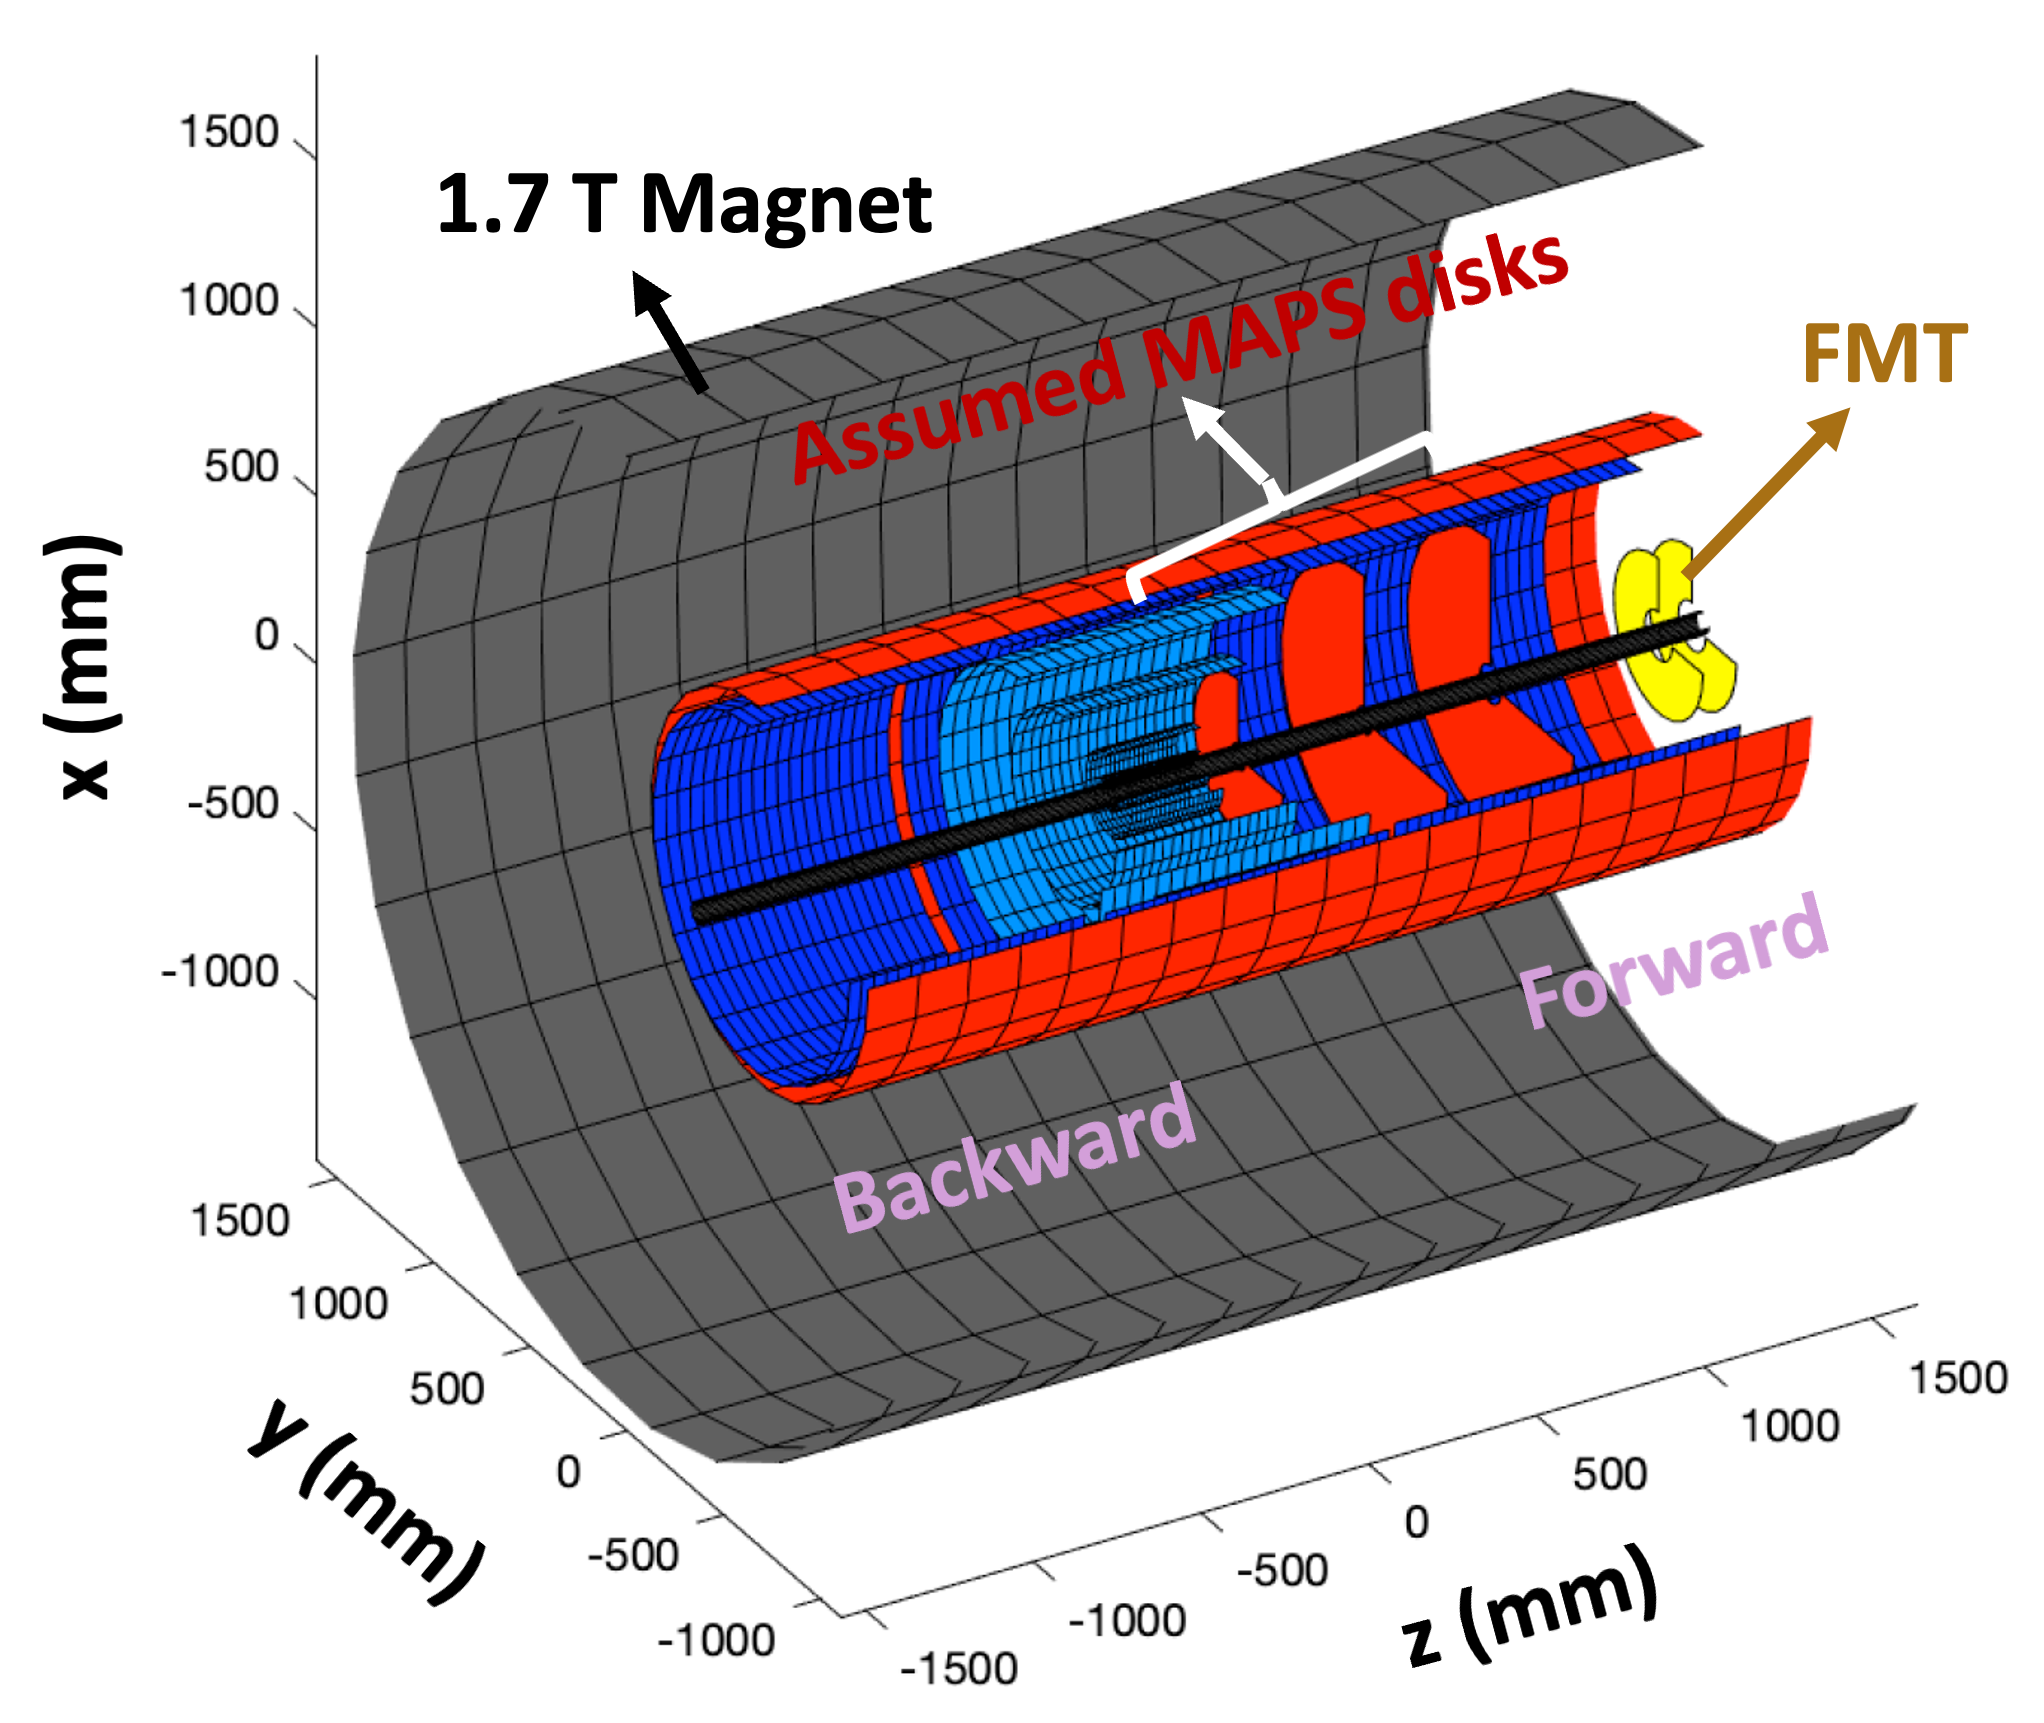
\includegraphics[width=0.8\linewidth]{FMT_geom.png}
\caption{Standalone simulation geometry showing the Fast MAPS Tracker (FMT, yellow) positioned downstream of the three MAPS tracking disks (red) within the ePIC solenoidal magnet (grey).}
\label{fig:fmt_geo}
\end{figure}

%\textcolor{red}{There are several overlap with the technology part, please revise the statement below.}
%The MALTA2 sensor used in this work is a monolithic CMOS silicon pixel detector designed in TowerJazz 180nm technology. This is the second prototype of monolithic active detectors in the MALTA family, prioritizing in-pixel charge collection efficiency and radiation hardness while reducing the cost and complexity of comparable hybrid sensors. Incident particles deposit charge into the depleted region of a MALTA2 pixel which is then collected by the small collection electrode for readout. The use of a smaller collection electrode than previous prototypes improves the signal to noise ratio and helps reduce random telegraph noise. \textbf{(Incident charged particles create electron-hole pairs in the depleted region of the silicon pixel. The resulting charge is then collected by the small collection electrode, whose low capacitance improves signal to noise ratio.} 

%\textcolor{red}{Please consider add figures of the MALTA2 sensors and MALTA2 quad-sensor module design.
%1. Technical design of the MALTA2 quad-sensor module.
%2. Layout and details of the design of the wire-bonds and readout components.
%3. Initial tests of the quad-sensor module.
%}

\subsection{MALTA2 quad-sensor module prototype design}

\begin{figure} [hbt]
    \centering
    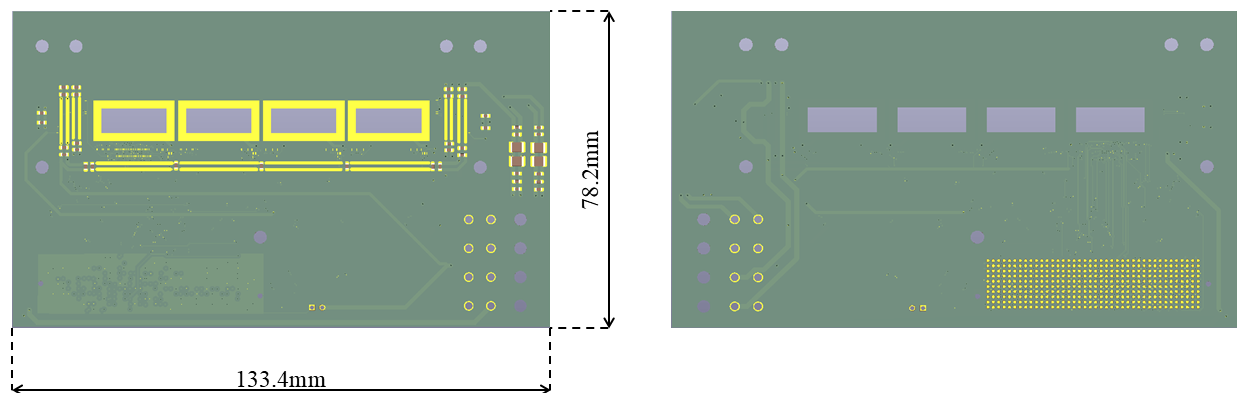
\includegraphics[width=1\linewidth]{PCB front and back.png}
    \caption{3D rendering of FMT MATLA2 Quad Module FPC prototype. The front view is shown in the left and the back view is shown in the right.}
    \label{fig:module_fpc}
\end{figure}

The MALTA2 quad-sensor module is designed as the fundamental building block of the FMT. As shown in Fig~\ref{fig:module_fpc}, four MALTA2 sensors are mounted side by side on the prototype Flexible Printed Circuit (FPC). 
The readout and power pads are located along both sides of the FPC, enabling the interconnection of multiple sensors to construct a larger detector matrix while providing flexibility in the placement of the master chip. In the slave-master readout architecture, all detector data are transmitted to and read out through the master chip. The master chip collects data from the upstream slave chips and output the aggregated data stream through the Low-Voltage Differential Signaling (LVDS) pads located on its bottom side, as seen in Fig~\ref{fig:module_electric}. This module design can minimize inter-chip communication distances while requiring only a single high-speed output link for the readout of the entire detector matrix. In the prototype carrier board used in this study, three slave chips are arranged in a row adjacent to the master chip, which is positioned on the left side of the module.

\begin{figure}[ht]
    \centering
    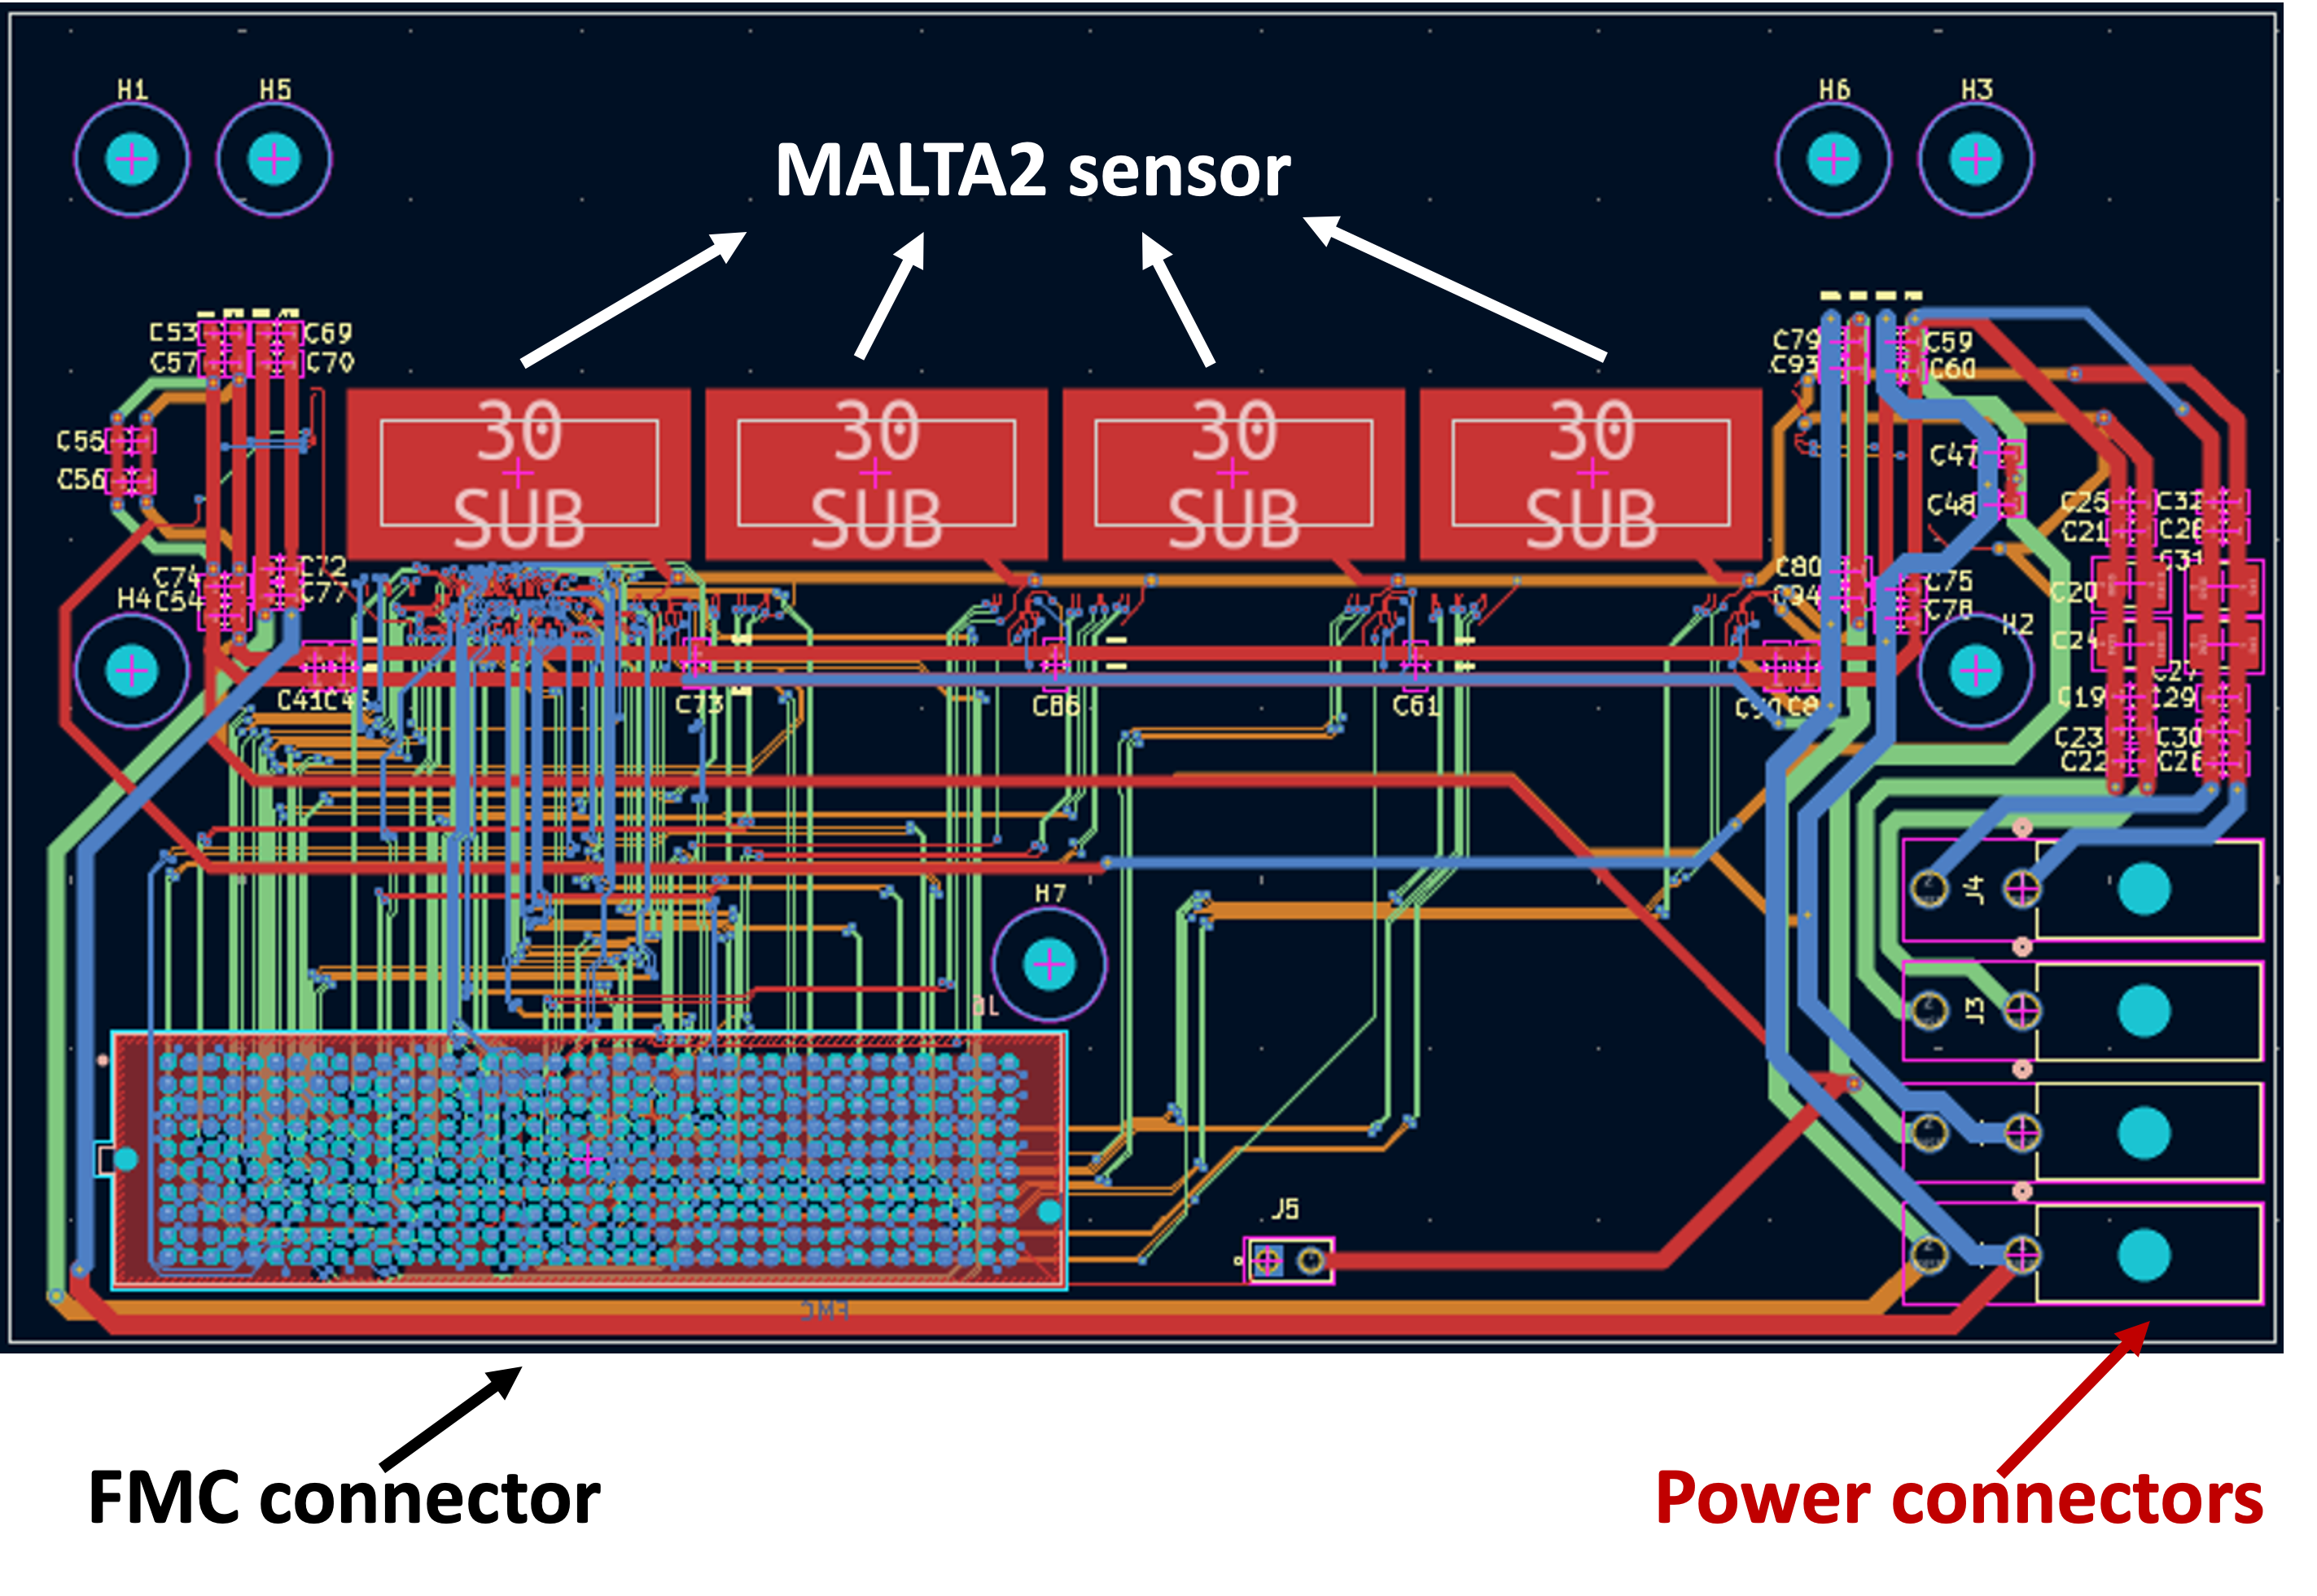
\includegraphics[width=0.9\linewidth]{MALTA2_module_electrical.png}
    \caption{Technical layout of the MALTA2 quad-sensor module prototype. The diagram illustrates the geometric arrangement of the four MALTA2 sensors, wire-bonding pads, and the routing paths for power distribution and high-speed differential signals.}
    \label{fig:module_electric}
\end{figure}

The MALTA2 sensors are integrated onto a custom-designed FPC that provides the mechanical support and electrical interfaces required for tracker operation. Owing to the small bond-pad dimensions ($88~\mu m \times 88~\mu m$) and fine pad pitch on both the sensors and the FPC, reliable chip-to-chip and chip-to-board interconnections are critical for the assembly of the modular. The FPC layout was optimized to ensure precise alignment of the electrical and mechanical components. The MALTA2 sensors were attached to the FPC using aluminum wedge wire bonding performed at the CERN Bonding Laboratory. Figure~\ref{fig:bond diagram} illustrates the wire-bonding scheme required for sensor operation. In this prototype, the leftmost sensor serves as the master chip, through which all detector readout and slow-control communication are routed, as reflected by the high density of wire bonds along its bottom edge.


\begin{figure}
    \centering
    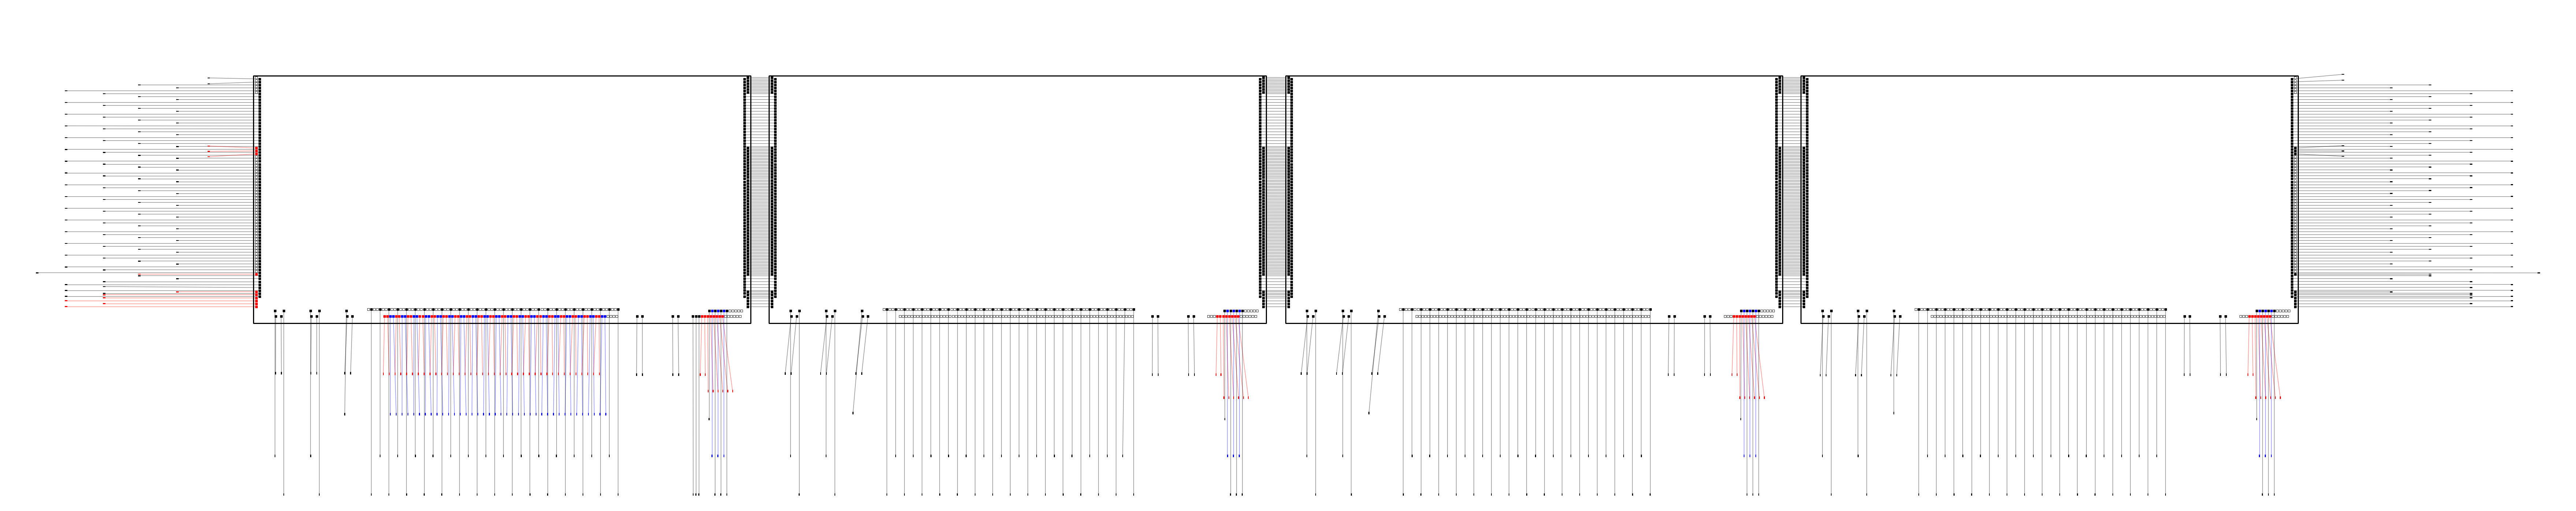
\includegraphics[width=1\linewidth]{QuadMod WireBond Clean.png}
    \caption{Schematic of the wire-bonding layout for the MALTA2 quad-sensor module.}
    \label{fig:bond diagram}
\end{figure}

%\textcolor{red}{To be merged with the readout section? Reference?}
%\textcolor{blue}{Kerem (10.08.2026): Agreed. I suggest merging this subsection with the Readout Firmware Development section to avoid repetition.}
%\textcolor{blue}{Kerem (10.08.2026): Another difference %from the single-chip readout is the extension from 37 to 38 LVDS inputs to include chip-identification information.}

%Is this the right idea for this section? how specific do we want
%LVDS readout/routing to the FMC? is it too much to discuss merging mechanics/the 37 bits of information that the LVDS outputs read?

\subsection{Initial Quad Module Testing}


%\begin{table}[h]
%\caption{Example of a lengthy table which is set to full textwidth}\label{tab2}
%\begin{tabular*}{\textwidth}{@{\extracolsep\fill}lcccccc}
%\toprule%
%& \multicolumn{3}{@{}c@{}}{Element 1\footnotemark[1]} & \multicolumn{3}{@{}c@{}}{Element 2\footnotemark[2]} \\\cmidrule{2-4}\cmidrule{5-7}%
%Project & Energy & $\sigma_{calc}$ & $\sigma_{expt}$ & Energy & $\sigma_{calc}$ & $\sigma_{expt}$ \\
%\midrule
%Element 3  & 990 A & 1168 & $1547\pm12$ & 780 A & 1166 & $1239\pm100$%\\
%Element 4  & 500 A & 961  & $922\pm10$  & 900 A & 1268 & $1092\pm40$\\
%\botrule
%\end{tabular*}
%\footnotetext{Note: This is an example of table footnote. This is an example of table footnote this is an example of table footnote this is an example of~table footnote this is an example of table footnote.}
%\footnotetext[1]{Example for a first table footnote.}
%\footnotetext[2]{Example for a second table footnote.}
%\end{table}


%\begin{figure}[h]
%\centering
%\includegraphics[width=0.9\textwidth]{fig.eps}
%\caption{This is a widefig. This is an example of long caption this is an example of long caption  this is an example of long caption this is an example of long caption}\label{fig1}
%\end{figure}


\section{MALTA2 quad-sensor module readout architecture and firmware development - (lead by Joellen, Kerem )}\label{sec:firm}

\subsection{Readout Architecture}
The MALTA2 quad-sensor module utilizes 38 Low-Voltage Differential Signaling (LVDS) pairs originating from the bottom side of the master chip. Each MALTA2 sensor comprises of 256 double column of pixels, which form the basis of the hierarchical data-merging architecture within the pixel matrix. When a hit is registered, the corresponding data propagates toward the end of the column as a 22-bit word, where the data-merging process begins. A hierarchy of eight merging stages consolidates the hit information from all 256 double columns into a 37-bit output word for transmission through the LVDS links, including a stage that combines the positive- and negative-parity groups within each double column. CMOS transistors located along the left and right edges of each chip enable data to be forwarded from the three secondary chips to the master chip, where the data streams are combined for final readout. The propagation delays associated with transferring data from the secondary sensors to the master chip are accounted for through the appropriate timing calibration/synchronization procedure. After the successive inter-chip merging stages are completed, the resulting data are transmitted through the LVDS links to the FPGA for further processing.

\subsection{Firmware Architecture}
The readout of the MALTA2 quad-module is being developed using the Alinx AXKU040 (Kintex UltraScale) platform. The custom FPGA design is based on a previous version that used the KC705 (Kintex 7) platform for readout of a single MALTA2 chip. 
% Kerem (10.08.2026):
% Original:
% Firmware updates have been made to target the new FPGA board and be able to control and read multiple chips.
%
% Revised:
Firmware updates were introduced to support quad-module operation by extending the data-input and slow-control interfaces while retaining the existing asynchronous readout architecture.

 
% Kerem (10.08.2026):
% Original:
% The FPGA receives data over the 37-bit bus of LVDS signals.
%
% Revised for quad-module operation:
For the quad-module implementation, the FPGA receives 38 differential signal pairs from the module. The additional information with respect to the single-chip readout provides the chip identification required to distinguish data originating from the four MALTA2 sensors. A two-bit chip identifier is associated with the data stream, with the values 00, 01, 10, and 11 identifying the four individual sensors. This allows data from all four MALTA2 chips to be transmitted through the common module readout path while preserving the identity of the sensor from which each hit originated.

The readout of the chips is fully asynchronous with no clock distribution needed between the chips and FPGA.
% Kerem (10.08.2026):
% Original:
% Each half of the differential signals are asynchronously oversampled using separate Input Delay Elements (IDELAYE) and Input Serializer/Deserializers (ISERDES) to achieve 8 samples from each pair. The reference clock used for the modules is 320MHz, which allows an effective sampling rate of 4GHz.
%
% Revised:
Each half of the differential signals is asynchronously oversampled using separate Input Delay Elements (IDELAYE) and Input Serializer/Deserializers (ISERDES). Using 640~MHz DDR sampling together with the independently delayed P and N signal paths, the implemented oversampling scheme achieves an effective sampling rate of 2.56~Gb/s.

Moving from the Kintex 7 platform to the Kintex UltraScale platform required updating the asynchronous sampling module to use IDELAYE3/ISERDES3 elements instead of IDELAYE2/ISERDES2 elements.

% Kerem (10.08.2026):
% Original:
% Slow control communication with the MALTA2 chips is done using the IPBUS protocol. Unlike the LVDS data signals, each chip requires its own slow control path. The Kintex 7 firmware slow control scheme was updated to add registers for each chip and add additional I/O for each chip.
%
% Revised:
Each MALTA2 sensor is configured through its dedicated slow-control interface, in which the configuration data are serially shifted into the on-chip configuration registers. For quad-module operation, separate slow-control data paths are provided for the four sensors, allowing the configuration of each chip to be programmed independently. This enables independent adjustment of the chip-level configuration parameters, including the programmable DAC settings, for each MALTA2 sensor.

\section{Performance Validation in Simulation - (Lead by Abhishek, Amelia, Lucian, Vlad)}\label{sec:mc}

The charge collection of the MALTA2 pixel has been derived from testbeam data \cite{MALTA2_CCParameterization}.
A parametric simulation approach is used that has been validated against data \cite{MALTAFastSim_Arxiv}.
A quad module made of four sensors in series simulated in GEANT4. Each sensor is identical but has time difference because of proximity (ref simulated geometry and schemtic). 
Characterization of sensors: Each sensor physical properties. 
fast simulation and Readout implementation(digitization) and tracking with custom configuration. 


\subsection{Telescope geometry and setup in simulation}
\begin{figure}[t]
    \centering
    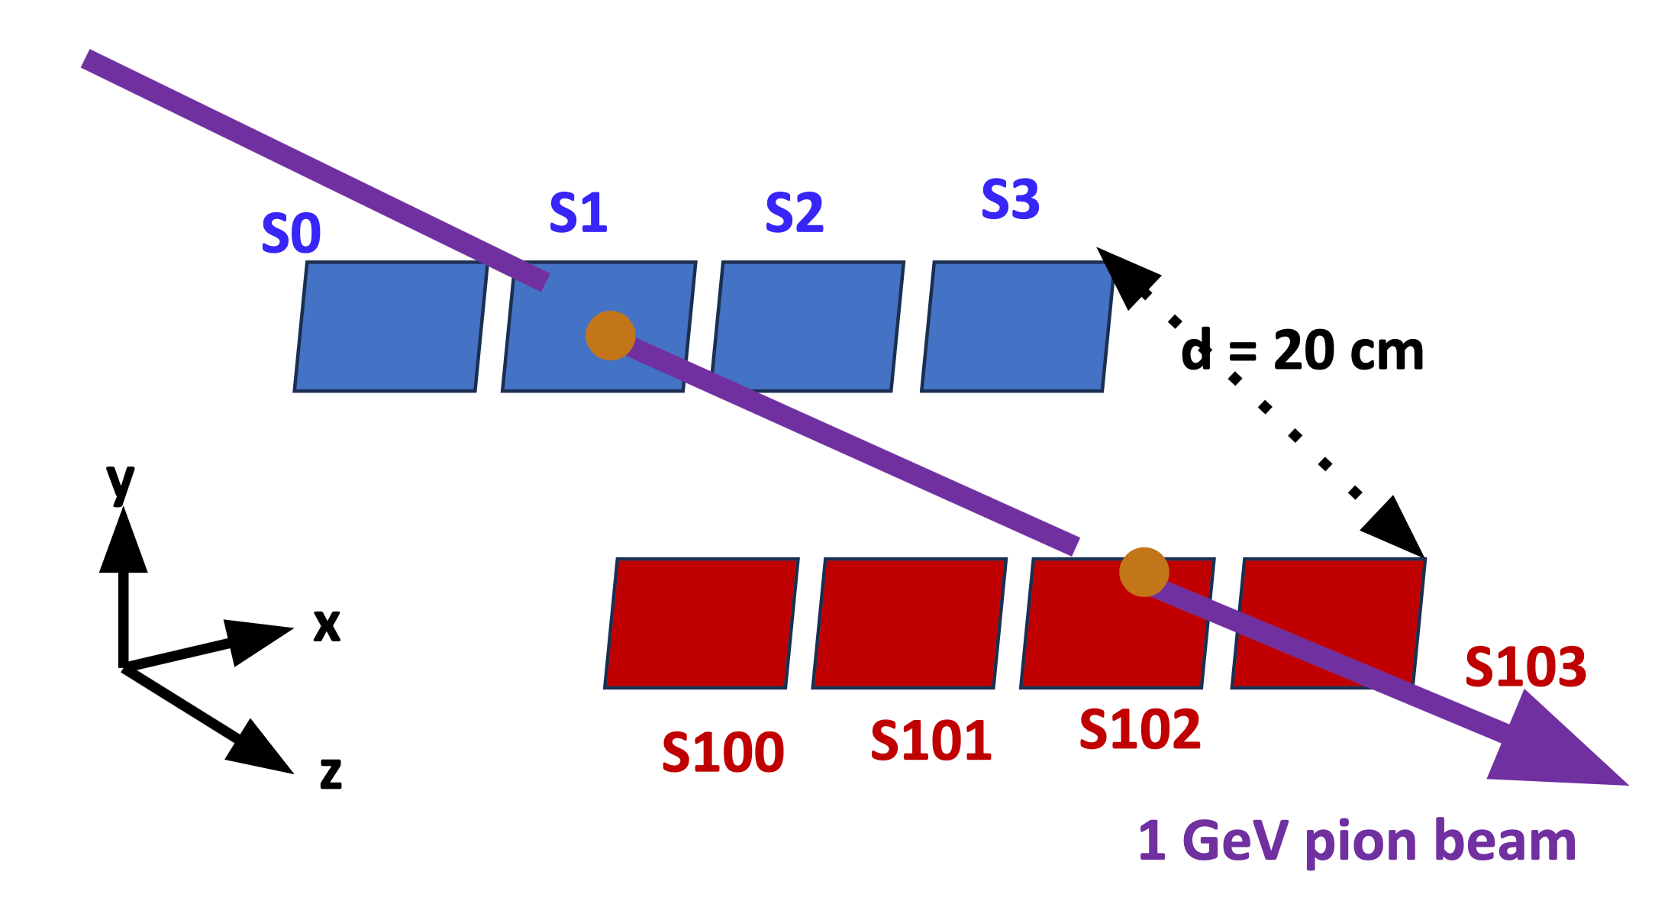
\includegraphics[width=0.9\linewidth]{Figures/geom.png}
    \caption{Telescope geometry and setup in simulation.}
    \label{fig:simgeom}
\end{figure}

The telescope is modelled in GEANT4 as a quad module of four identical
MALTA2 sensors placed in series along the beam axis. Each sensor is a
$1.8\times0.9~cm^2$ monolithic CMOS pixel matrix with a
pixel pitch of \SI{36.4}{\micro\meter}, giving a $512\times224$ pixel grid.
The sensors are separated by a fixed spacing, so a particle crosses the
planes sequentially. Small time offsets between planes, arising from their
relative position and readout propagation, are applied per sensor.

Primaries are generated per event with a configurable multiplicity. The
first primary in each event is the signal (a \SI{1}{\GeV} $\pi^{+}$)
incident perpendicular to the sensor plane; any additional primaries are
background (\SI{10}{\MeV} $e^{-}$). Each primary is placed at a random
position within the active area and assigned a global time
$t = N_\text{evt}\,t_\text{veto} + \delta t$, where $N_\text{evt}$ is the
event index and $\delta t$ is a random intra-spill offset up to
\SI{2}{\micro\second}. Signal and background therefore overlap in time and
are distinguished only by their truth label, not by arrival time.

Energy deposition in each sensor is digitized with the parametric MALTA2
response (charge collection, threshold, and timing), and the resulting
pixel hits are reconstructed per plane. Truth provenance
(event ID and track ID) is propagated through digitization to allow exact
signal-to-hit association for the efficiency and tracking studies that
follow.

\subsection{Time Resolution (no background)}
\textcolor{red}{Plot: Time resolution (compare: without background, with 1,2,3 particles per event)}
Validated with data.

\subsection{Background rate}
Explain the expected background at the location of the FMT (from Amelia's plots?):
\begin{itemize}
    \item Select region of $1\times\SI{2}{\square\centi\meter}$ with highest hit rate.
    \item Show distribution of hits per $\SI{2}{\micro\second}$ event
    \item Show PDG code of background particles. Is it primarily photons and electrons/ positrons?
\end{itemize}

Explain the simplifications/ assumptions that go into the MALTA2 simulation.
\begin{itemize}
    \item Identify maximum expected background hit rate per sampled event.
    \item Spatial distribution is approximately flat within individual MALTA2 sensor.
\end{itemize}

\subsection{Hit efficiency with background}
\textcolor{red}{Plot: Hit efficiency of a signal particle versus background rate per event:}
\begin{itemize}
    \item Position of background and signal is random in MALTA2 sensor.
    \item Keep time window of background particles within \SI{10.2}{\nano\second}.
    \item Increase number of background particles that fall within this. (Expectation from Lucian: Efficiency is still >90\% for 1,2,3 background particles but decreases drastically for >3 particles.
\end{itemize}



\subsection{Tracking efficiency, potential spatial/temporal resolution with background}
This subsection can target the proper tracking efficiency using 2 FMT planes.
\begin{itemize}
    \item Obtain hits per plane.
    \item Reconstruct a track from the two planes.
    \item Calculate pointing resolution of the track. In the simulation, signal is incident perpendicular onto the sensor. How is the direction reconstructed from the track?
\end{itemize}

\subsection{Matching capability with background}


\section{Summary}\label{sec:sum}

Conclusions may be used to restate your hypothesis or research question, restate your major findings, explain the relevance and the added value of your work, highlight any limitations of your study, describe future directions for research and recommendations. 

In some disciplines use of Discussion or 'Conclusion' is interchangeable. It is not mandatory to use both. Please refer to Journal-level guidance for any specific requirements. 


\section*{Acknowledgment}
This material is based upon work supported by the U.S. Department of Energy, Office of Science, Office of Nuclear Physics under Award Number DE-SCL0000067. This work was supported in part by the U.S. Department of Energy, Office of Science, Office of Workforce Development for Teachers and Scientists (WDTS) under the Science Undergraduate Laboratory Internships (SULI) program. Part of the research presented in this article was supported by the Laboratory Directed Research and Development program of Los Alamos National Laboratory under project number 20260377ER.


%%================================%%
%% Sample for structured abstract %%
%%================================%%

% \abstract{\textbf{Purpose:} The abstract serves both as a general introduction to the topic and as a brief, non-technical summary of the main results and their implications. The abstract must not include subheadings (unless expressly permitted in the journal's Instructions to Authors), equations or citations. As a guide the abstract should not exceed 200 words. Most journals do not set a hard limit however authors are advised to check the author instructions for the journal they are submitting to.
% 
% \textbf{Methods:} The abstract serves both as a general introduction to the topic and as a brief, non-technical summary of the main results and their implications. The abstract must not include subheadings (unless expressly permitted in the journal's Instructions to Authors), equations or citations. As a guide the abstract should not exceed 200 words. Most journals do not set a hard limit however authors are advised to check the author instructions for the journal they are submitting to.
% 
% \textbf{Results:} The abstract serves both as a general introduction to the topic and as a brief, non-technical summary of the main results and their implications. The abstract must not include subheadings (unless expressly permitted in the journal's Instructions to Authors), equations or citations. As a guide the abstract should not exceed 200 words. Most journals do not set a hard limit however authors are advised to check the author instructions for the journal they are submitting to.
% 
% \textbf{Conclusion:} The abstract serves both as a general introduction to the topic and as a brief, non-technical summary of the main results and their implications. The abstract must not include subheadings (unless expressly permitted in the journal's Instructions to Authors), equations or citations. As a guide the abstract should not exceed 200 words. Most journals do not set a hard limit however authors are advised to check the author instructions for the journal they are submitting to.}


\appendix

\section{Appendix section}\label{app}

We consider a sequence of queueing systems
indexed by $n$.  It is assumed that each system
is composed of $J$ stations, indexed by $1$
through $J$, and $K$ customer classes, indexed
by $1$ through $K$.  Each customer class
has a fixed route through the network of
stations.  Customers in class
$k$, $k=1,\ldots,K$, arrive to the
system according to a
renewal process, independently of the arrivals
of the other customer classes.  These customers
move through the network, never visiting a station
more than once, until they eventually exit
the system.

%%===========================================================================================%%
%% If you are submitting to one of the Nature Portfolio journals, using the eJP submission   %%
%% system, please include the references within the manuscript file itself. You may do this  %%
%% by copying the reference list from your .bbl file, paste it into the main manuscript .tex %%
%% file, and delete the associated \verb+\bibliography+ commands.                            %%
%%===========================================================================================%%

% BibTeX users please use one of
%\bibliographystyle{spbasic}      % basic style, author-year citations
%\bibliographystyle{spmpsci}      % mathematics and physical sciences
\bibliographystyle{spphys}       % APS-like style for physics
\bibliography{Fmtref}   % name your BibTeX data base


\end{document}
